
Two-Level Segregated Fit (TLSF) is a dynamic storage allocator developed by M. Masmano et al.~\cite{TLSF}. It is especially designed to be used in real-time applications, where it stands out among other allocators in that it has a bounded and short response time and maintaining low fragmentation, thus ensuring high predictability. 

The work of the TLSF authors primarily concentrate on low-level allocation primitives, without explicit consideration for garbage collection. Consequently, exploring the adaptation of TLSF to integrate with a garbage collector represents a direction for advancing its development.

The name TLSF reflects its design as a free-list based allocator that uses segregated-fit, storing multiple free-lists containing blocks of set size classes. To efficiently lookup what free-list contain blocks, TLSF employs two levels of bitmaps. The first level bitmap for size classes that are separated by powers of two called first-level, and a second-level that subdivides the first-level size classes linearly. In the reference implementation, the number of first- and second-levels are both limited to 32 in order to fit in 32-bit values. Additionally, the number of second-levels are recommended to be a power of two for efficiency reasons, so that simple bit instructions can be used.

Allocations inside TLSF are managed using blocks. Blocks are managed using two doubly-linked list structures. Initially, blocks are arranged in a physically ordered list, and if a block becomes free, it is then inserted into an appropriate free-list. Each block is accompanied by an associated header located next to it. The header specifies the size of the block and also its position within both doubly-linked lists. There is a slight difference of what the header contains depending on if the block is free or not, where free blocks contain additional metadata, as shown in Figure~\ref{fig:blockheader_reference}. Moreover, block sizes are aligned to multiples of four to align with the allocation unit (4 bytes for a 32-bit architecture). The two least significant bits within the block header are reserved for metadata. These bits indicate whether the block is free (F-bit) and whether it represents the last block within its pool (L-bit), as depicted in Figure~\ref{fig:blockheader_reference}. The F-bit is mainly used to see if a block is free and can be coalesced and the L-bit is used to easily iterate over physical blocks.

% Explain L-bit, explain what blocks are and that there initially exists one large block.

% TODO: Fix correct citation for figure?
\begin{figure}[H]
    \centering
    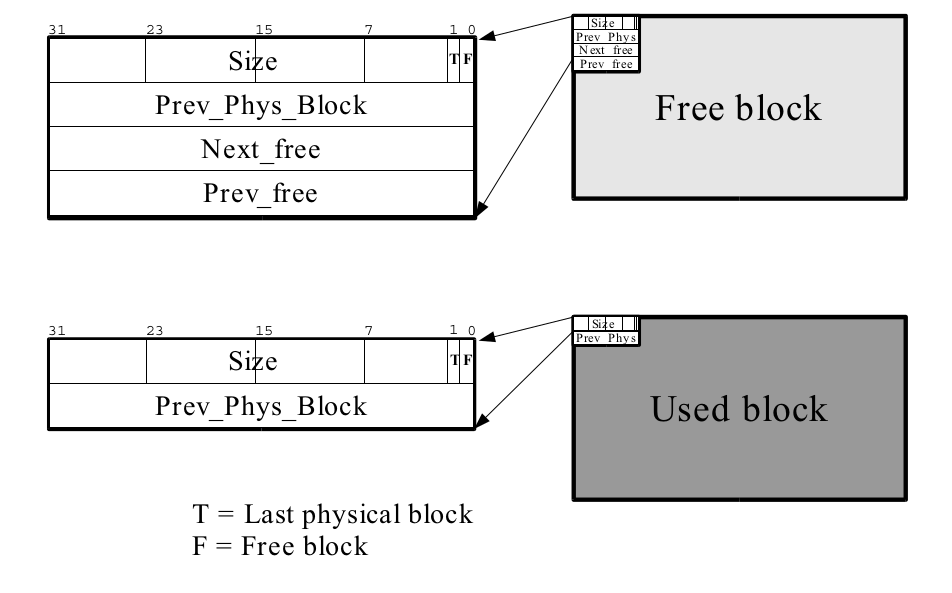
\includegraphics[width=0.65\textwidth]{figures/blockheader_reference.png}
    \caption{Representation of free and allocated block headers in 32-bit architecture. For a 64-bit architecture, each individual field is 8 bytes instead of 4 bytes. (Taken from~\cite{TLSF}).}
    \label{fig:blockheader_reference}
\end{figure}

\subsection{Allocation and Freeing Strategy}

While from the user's perspective, TLSF behaves similarly to familiar memory allocation and deallocation functions like malloc/free in libc\footnote{See the Linux Programmer's Manual for more information on `malloc()` and `free()`. Accessed online at: \url{https://man7.org/linux/man-pages/man3/malloc.3.html}}, its distinctive characteristics lie in its internal mechanisms, which will be discussed next.

When a user requests N bytes from the allocator, the allocator aligns N to meet any necessary alignment requirements and applies padding. Subsequently, it searches for a block matching the desired size. If no block within the specific size range is found, the allocator continues its search to identify a larger block. If no block is found, a NULL value is returned. However, if a list containing blocks is found, the allocator picks the first block in the list, regardless of the number of blocks in it. The policy of searching for free-lists and choosing the first block is called Good-Fit by the authors, referred to as a combination of best- and first-fit. This policy was chosen since it performs well in terms of fragmentation. Moreover, if a block larger than the requested size is located, the allocator splits it into two blocks. One block is used to satisfy the request to the user, and the other is inserted back into the allocator.

Later on, when a user decides to free an allocated block, it is implicitly attempted to be coalesced, or merged, with the block(s) that are located adjacent to it in physical order. The reason for coalescing immediately when freeing is to be able to have larger blocks available for larger requests sizes as often as possible. This is because external fragmentation is minimized if we aim toward having as few small blocks as possible.

%%% Local Variables:
%%% mode: latex
%%% TeX-master: "main"
%%% End:
